\documentclass[twocolumn, aps, apl]{revtex4-1}

\usepackage{graphicx}
\usepackage{fancyhdr}
\usepackage{amsmath}
\usepackage{caption}
\usepackage{enumerate}
\usepackage{subcaption}
\usepackage{textcomp}
\usepackage{placeins}

\begin{document}
\title{Lab 1. S Parameter and Spectral Measurements of Microwave Amplifiers}
\author{Albert Wandui}
\affiliation{EE 152: High Frequency Systems Lab.}
\maketitle

\section*{Introduction}
The goal of this lab was to characterize the output power capabilities of a microwave amplifier using both a Network and Spectrum Analyzer. Network Analyzers (NAs) are useful for measuring the S parameters of a device under test (DUT). This makes them indispensible in designing RF and Microwave Systems. In order to make reliable measurements using the NA, the device must first be calibrated by measuring the S parameters of a precision standard. This was the first goal of this lab. Once the calibration is performed, the NA can be used to measure both the magnitude and phase of the S parameters of the amplifier over a defined frequency band. The Field Fox NA is a Vector Network Analyzer (VNA). This means that it can measure both the Magnitude and Phase of the S parameters.

In contrast to the NA, the Spectrum Analyzer (SA) is a single port device and measures the output power of a device under test as a function of the frequency. Spectrum Analyzers are useful for measuring the Signal to Noise Ratio (SNR) for DUTs under particular input power and biasing conditions. They are also useful in understanding non-linearities in electrical components. For linear devices powered at a particular frequency, the output response is also at the same frequency. However, non-linearities in a device (in this case the amplifier) can excite the harmonics of the fundamental mode. 


\section*{Calibration Measurements}
For the calibration measurements, we used for precision calibration standards; open, short, load and through. We performed a full 2 port calibration measurement by connecting each of the calibration standards to port 1 and measuring the S parameters and repeating the entire process on port 2 of the NA as well. Care was taken to ensure that the SMA connectors were hand-tight to prevent damage to the connectors. In addition, we ensured that all the cables were connected through connect 'savors` at their ends to prevent possible damage to expensive cables and devices. For our measurements, the NA analyzer was used in a frequency band between 100 MHz and 18GHz for all the measurements. The IF Bandwidth was set to 10 kHz. The choice of the IF Bandwidth impacts the amount of time needed to perform the measurements. We also critically, set the input power to -30 dBm to ensure that the power level was low enough that the amplifier output would not damage the NA. The input power level was set to ensure a good balance between accuracy in measurement and safety in operating the NA when measuring an active device. 

One key goal of this section of the lab was to build an understanding of reference plane extension concepts. All S parameter measurements are measured with respect to a particular point in the circuit which is called the reference plane. For the NA, the reference plane is defined to be at the interface of the NA cables following calibration. Changing the position of the reference plane shifts the phase of the S parameters. For our calibration measurements, a reference plane extension was needed because the shorted plane of the calibration standard did not coincide with the defined reference plane of the NA. To adjust the reference plane, a phase must be added to the S-parameters. The phase $\phi$ added is given by the distance between the two reference planes $l$ by the relation $\phi = 2 \pi c \tau/l$ where $\tau$ is the time delay for the input wave to travel between the two reference planes and c is the speed of light.  Ideally, on a Smith Chart, the short calibration standard should be a single point at the 9 o'clock position for all frequencies. However, without the reference plane extension, each frequency within the band acquires a different phase shift and the single point at the 9 o'clock position is smeared out to cover the entire circumference of the Smith Chart. The reference plane is thus adjusted until all the points are centered back on the 9 o'clock position. When we did this, we measured $\tau = 32 ps$ giving $l = 9.593 mm$.

The same reference plane extension can be achieved by adding a suitable length of transmission line to the input port of the DUT to provide the needed phase delay. In Microwave Office, you can emulate this by adding a transmission line of a given impedance and phase velocity and adjusting its length to obtain the desired phase. Microwave Office allows the value of the length parameter to be negative to account for both positive and negative phase shifts. To emulate the ref plane extension in Microwave Office, I added a section of 50 $\Omega$ transmission line with a length of -377.7 mils to the input of the short calibration standard. The figure \ref{fig:calib} shows the match between the reference plane extension done on the NA and the emulated version from Microwave Office.

\begin{figure}[!htbp]
    \centering
    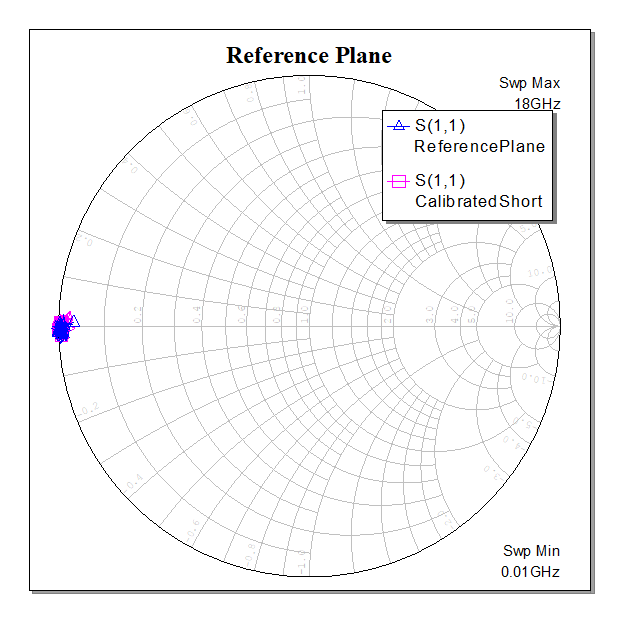
\includegraphics[scale=0.5]{CalibratedShort.png}
    \caption{Smith Chart showing the Short Calibration Standard with Reference Plane Extensions done on the NA (purple) and emulated on Microwave Office (blue).}
    \label{fig:calib}
\end{figure}

\FloatBarrier

\section*{S Parameter Measurements}

The figure \ref{fig:ampimg} shows the experimental setup used to measure the amplifier S parameters on the NA. The amplifier was biased at 5.00 V and 70 mA for all the measurements. In addition, we set the over voltage protection (OVP) to 5.5 V and the over current protection (OCP) to 100 mA. These two limits prevent the amplifier from exceeding its design current and voltage limits. The VNA was allowed to sweep multiple times and the 4 2 port S parameters were measured. The amplifier measurements showed good match with the response specified in the amplifier datasheet. The comparison plots are shown in figure \ref{fig:amp}. The key differences are the presence of noise fluctuations in the VNA measurements as well as intermittent dips in the response especially in the $S_{22}$ parameter. These dips are likely a result of stray frequency dependent impedances that introduce additional reflections that suppress the response at particular frequencies. These stray impedances are likely due to the connectors used to attach the components.

\begin{figure}[!htbp]
    \centering
    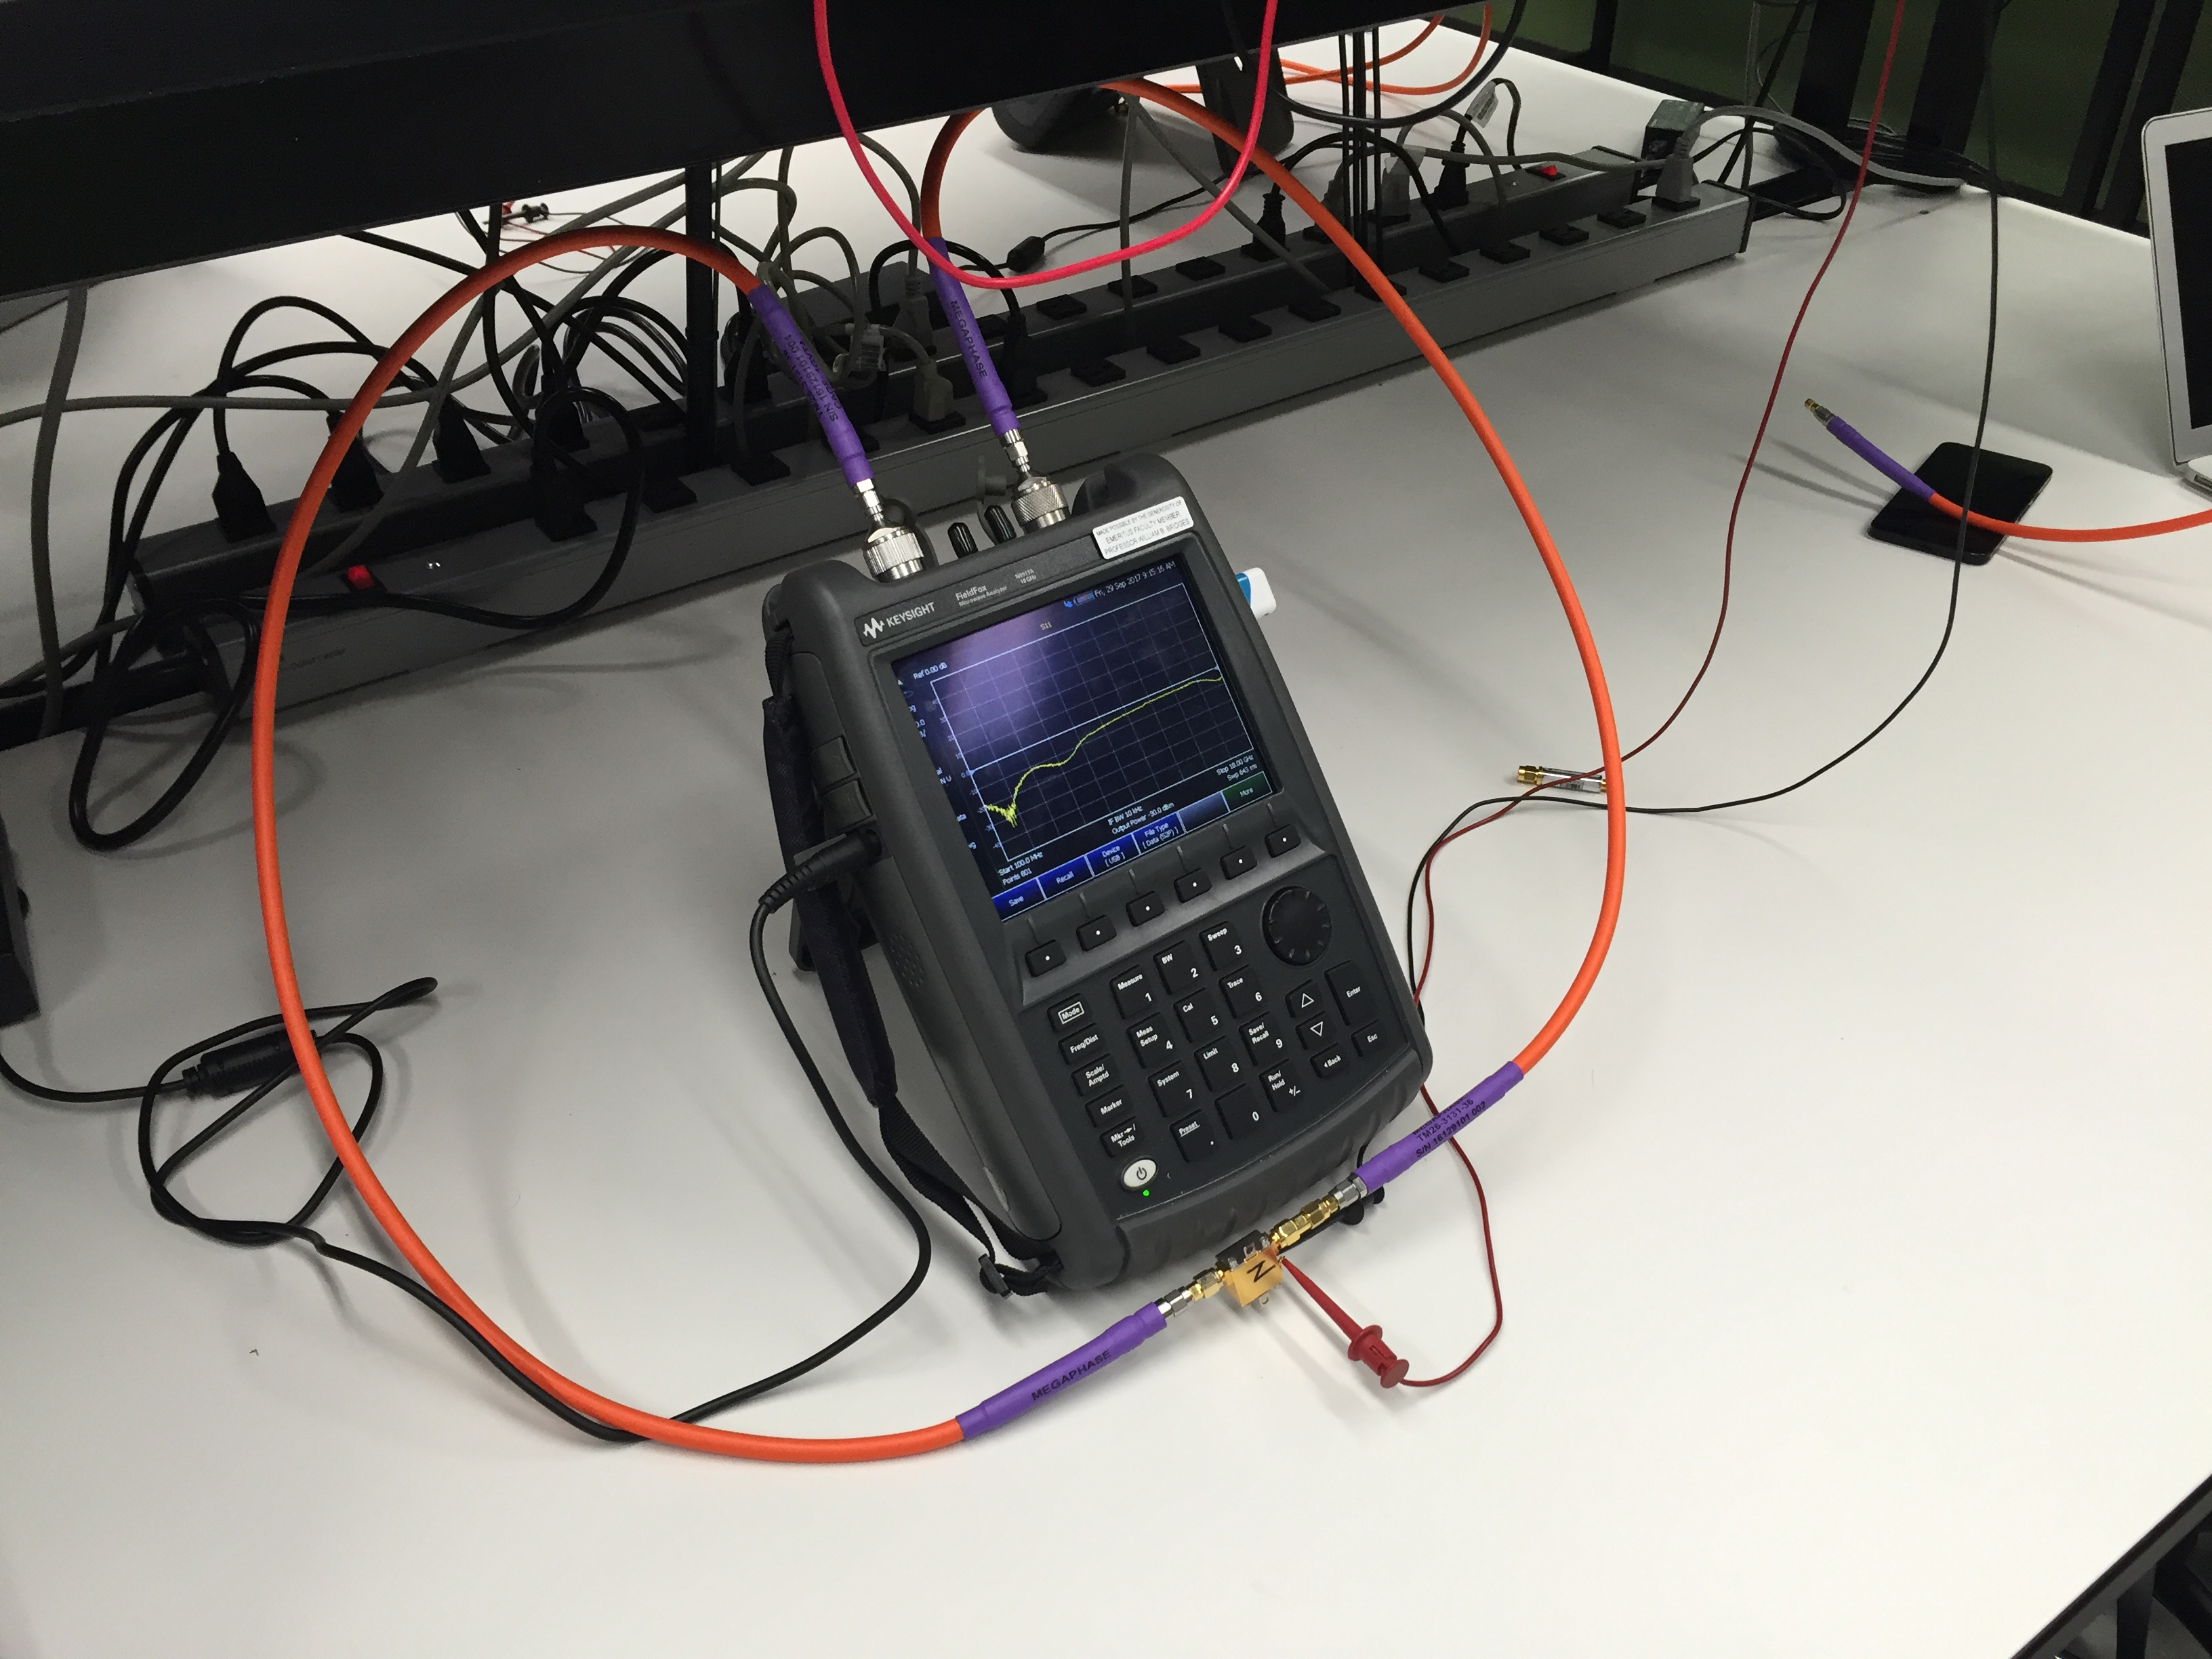
\includegraphics[width=0.35\textwidth]{amp_measurement.jpeg}
    \caption{Measurement Setup for amplifier on the NA.}
    \label{fig:ampimg}
\end{figure}


\begin{figure}[!htbp]
    \centering
    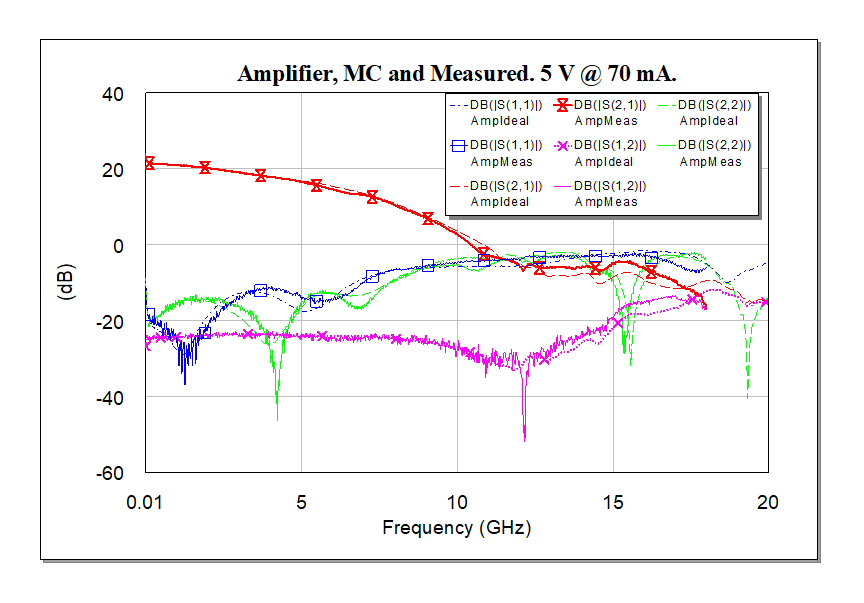
\includegraphics[scale=0.45]{AmplifierMCandMeasured.png}
    \caption{Comparison of the Amplifier S parameters from the NA measurements to the sourced values from the data sheet.}
    \label{fig:amp}
\end{figure}

We also performed S parameter measurements of the filter using the circuit shown in figure \ref{fig:filterimg} and with the response shown in figure \ref{fig:filter}. Note that the filter is a passive device and its scattering matrix is reciprocal i.e. $S_{21} = S_{12}$ unlike the amplifier. The bandpass filter has a flat forward response in band (about 4.9 - 6 GHz).
\begin{figure}[!htbp]
    \centering
    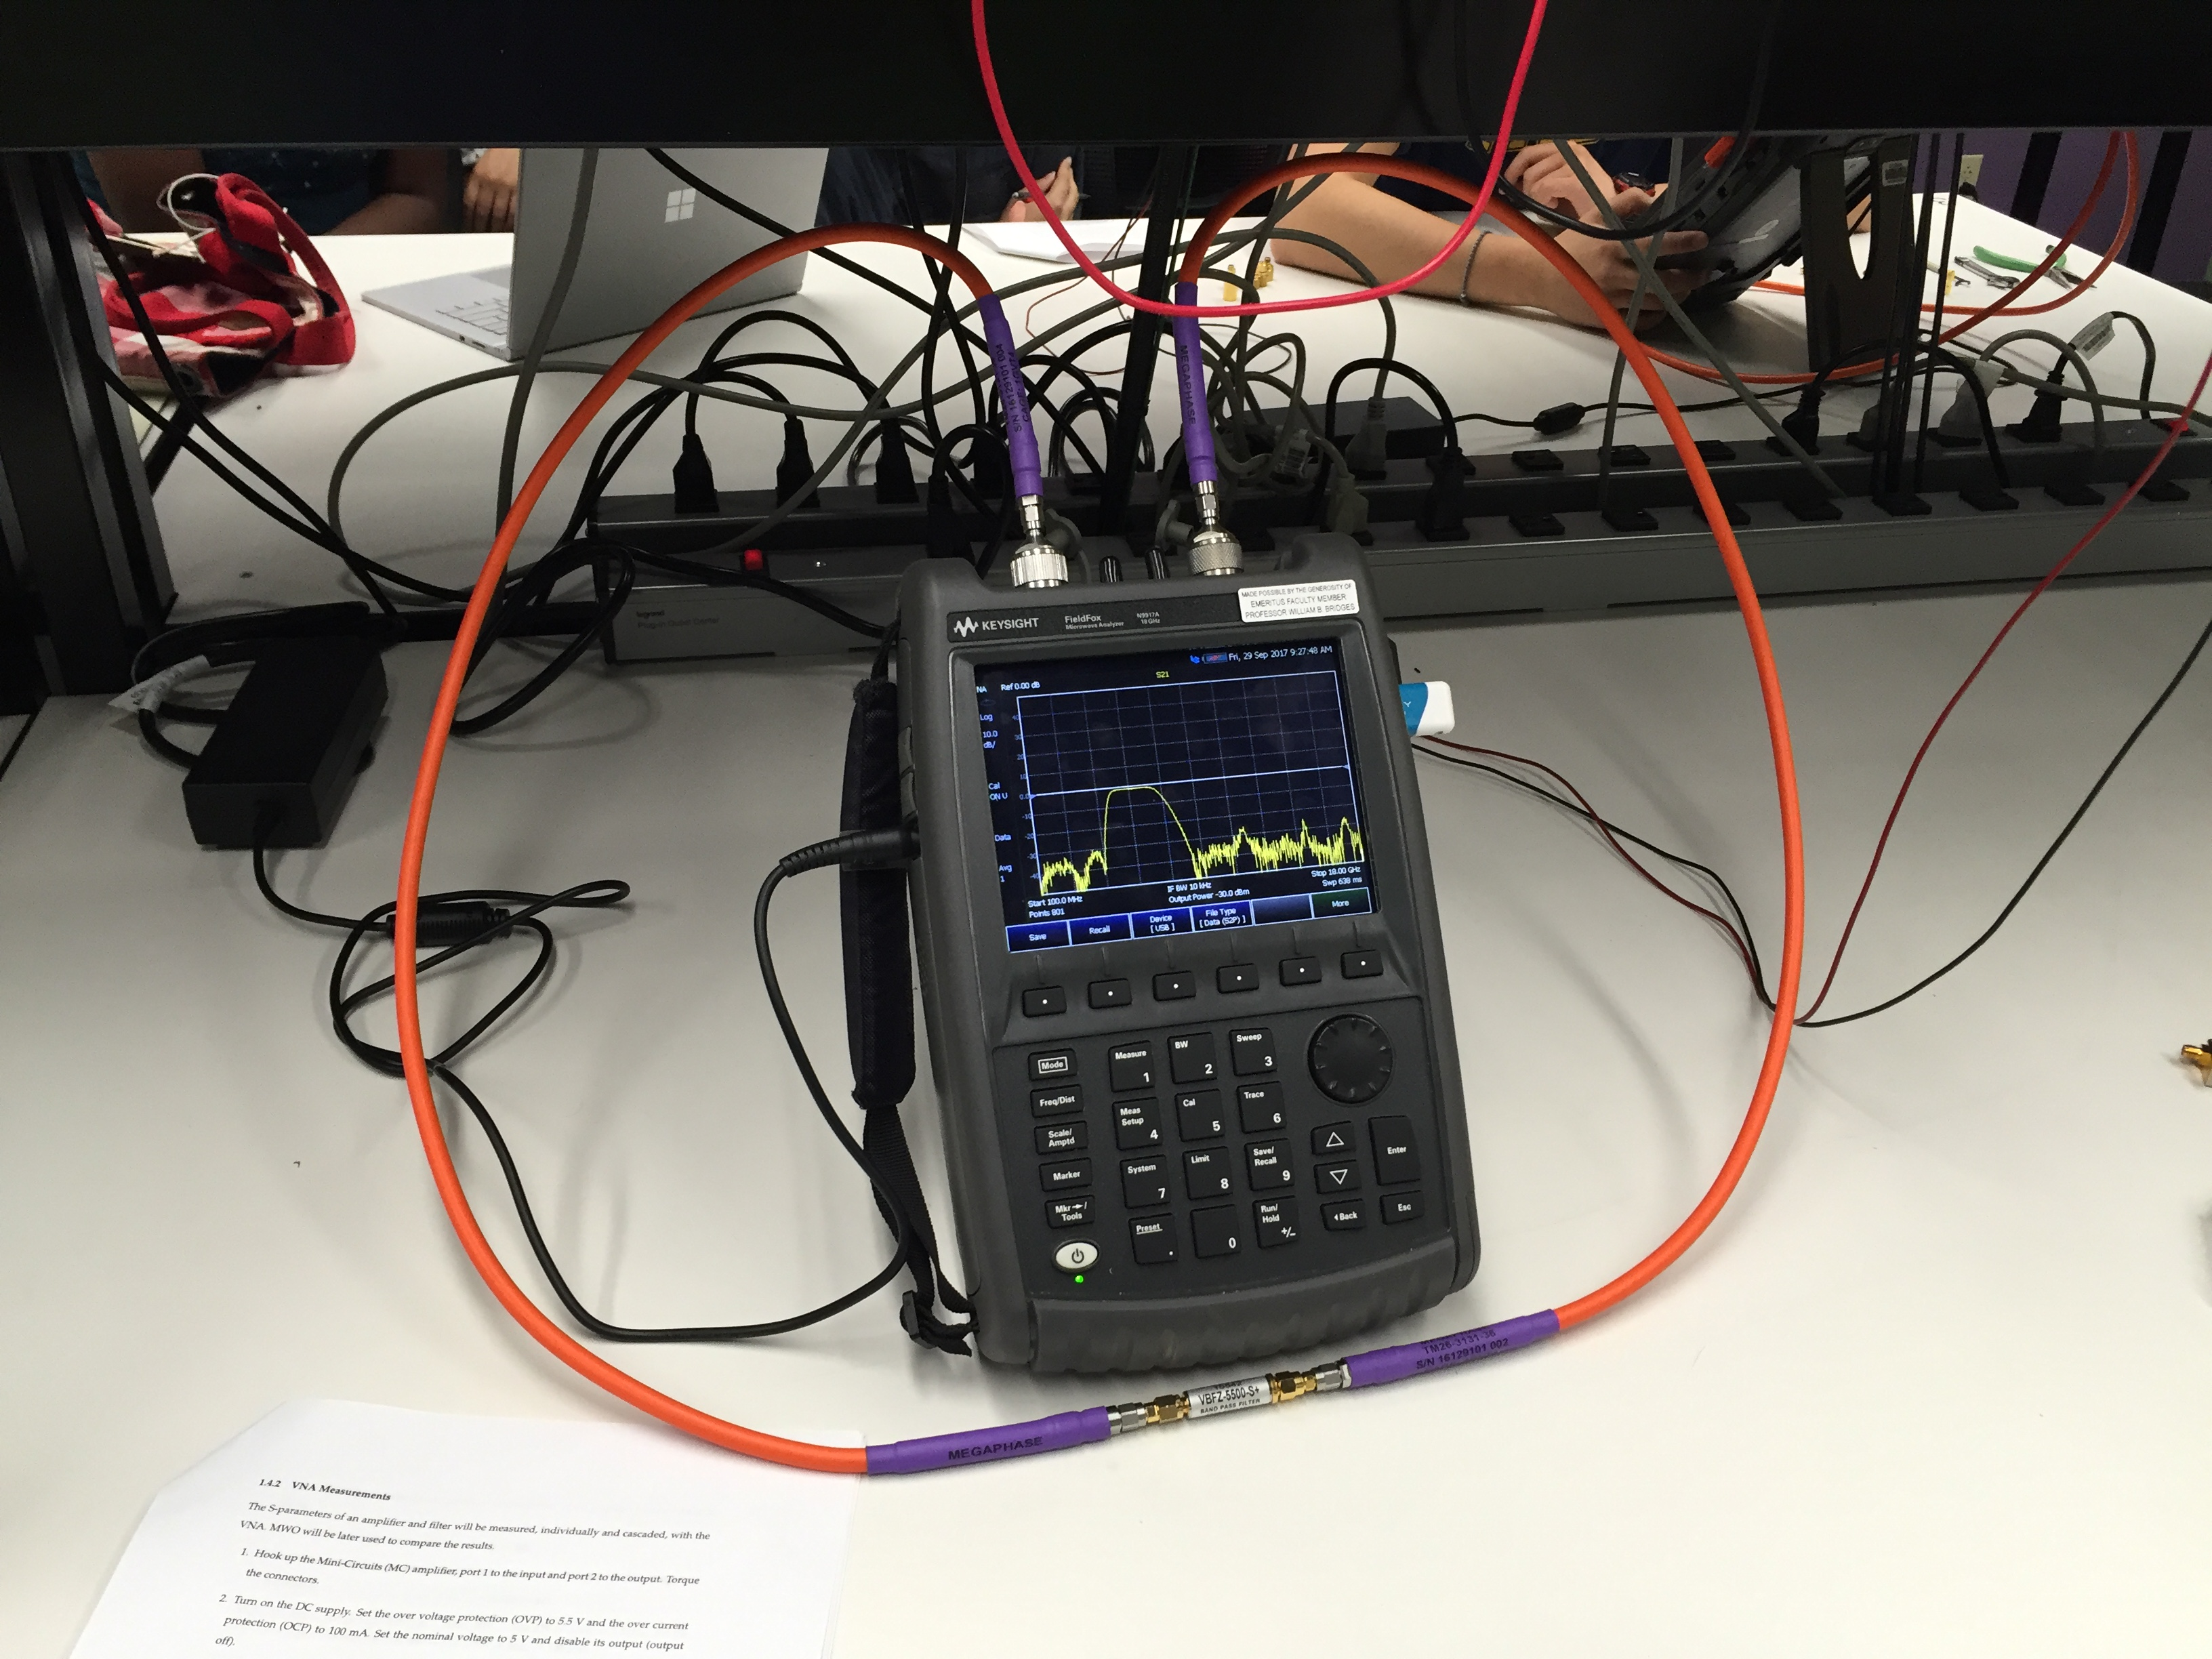
\includegraphics[width=0.35\textwidth]{filter_measurement.jpeg}
    \caption{Measurement Setup for filter on the NA.}
    \label{fig:filterimg}
\end{figure}


\begin{figure}[!htbp]
    \centering
    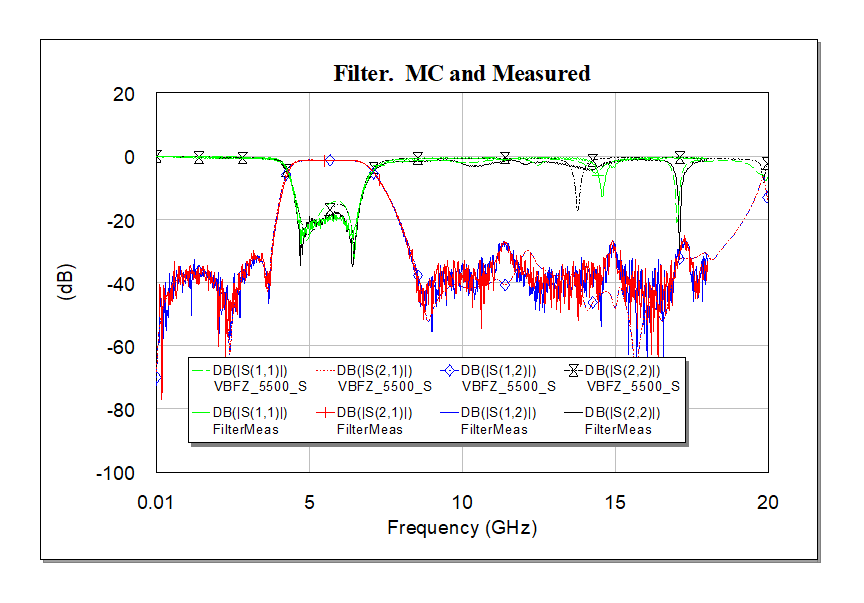
\includegraphics[scale=0.45]{FilterMCandMeasured.png}
    \caption{Comparison of the Filter S parameters from the NA measurements to the sourced values from the data sheet.}
    \label{fig:filter}
\end{figure}

With the filter circuit added to the output of the amplifier, the response of the amplifier is shaped by the transfer function of the filter. The experimental setup is shown in figure \ref{fig:filterampimg} and the combined amplifier and filter response as measured vs. the simulated response is shown in figure \ref{fig:ampfilter}. The filter acts as a bandpass suppressing amplifier transmission below about 4.9 GHz and above about 6 GHz. The out of band sidelobes in the frequency response are also clearly visible.
\begin{figure}[!htbp]
    \centering
    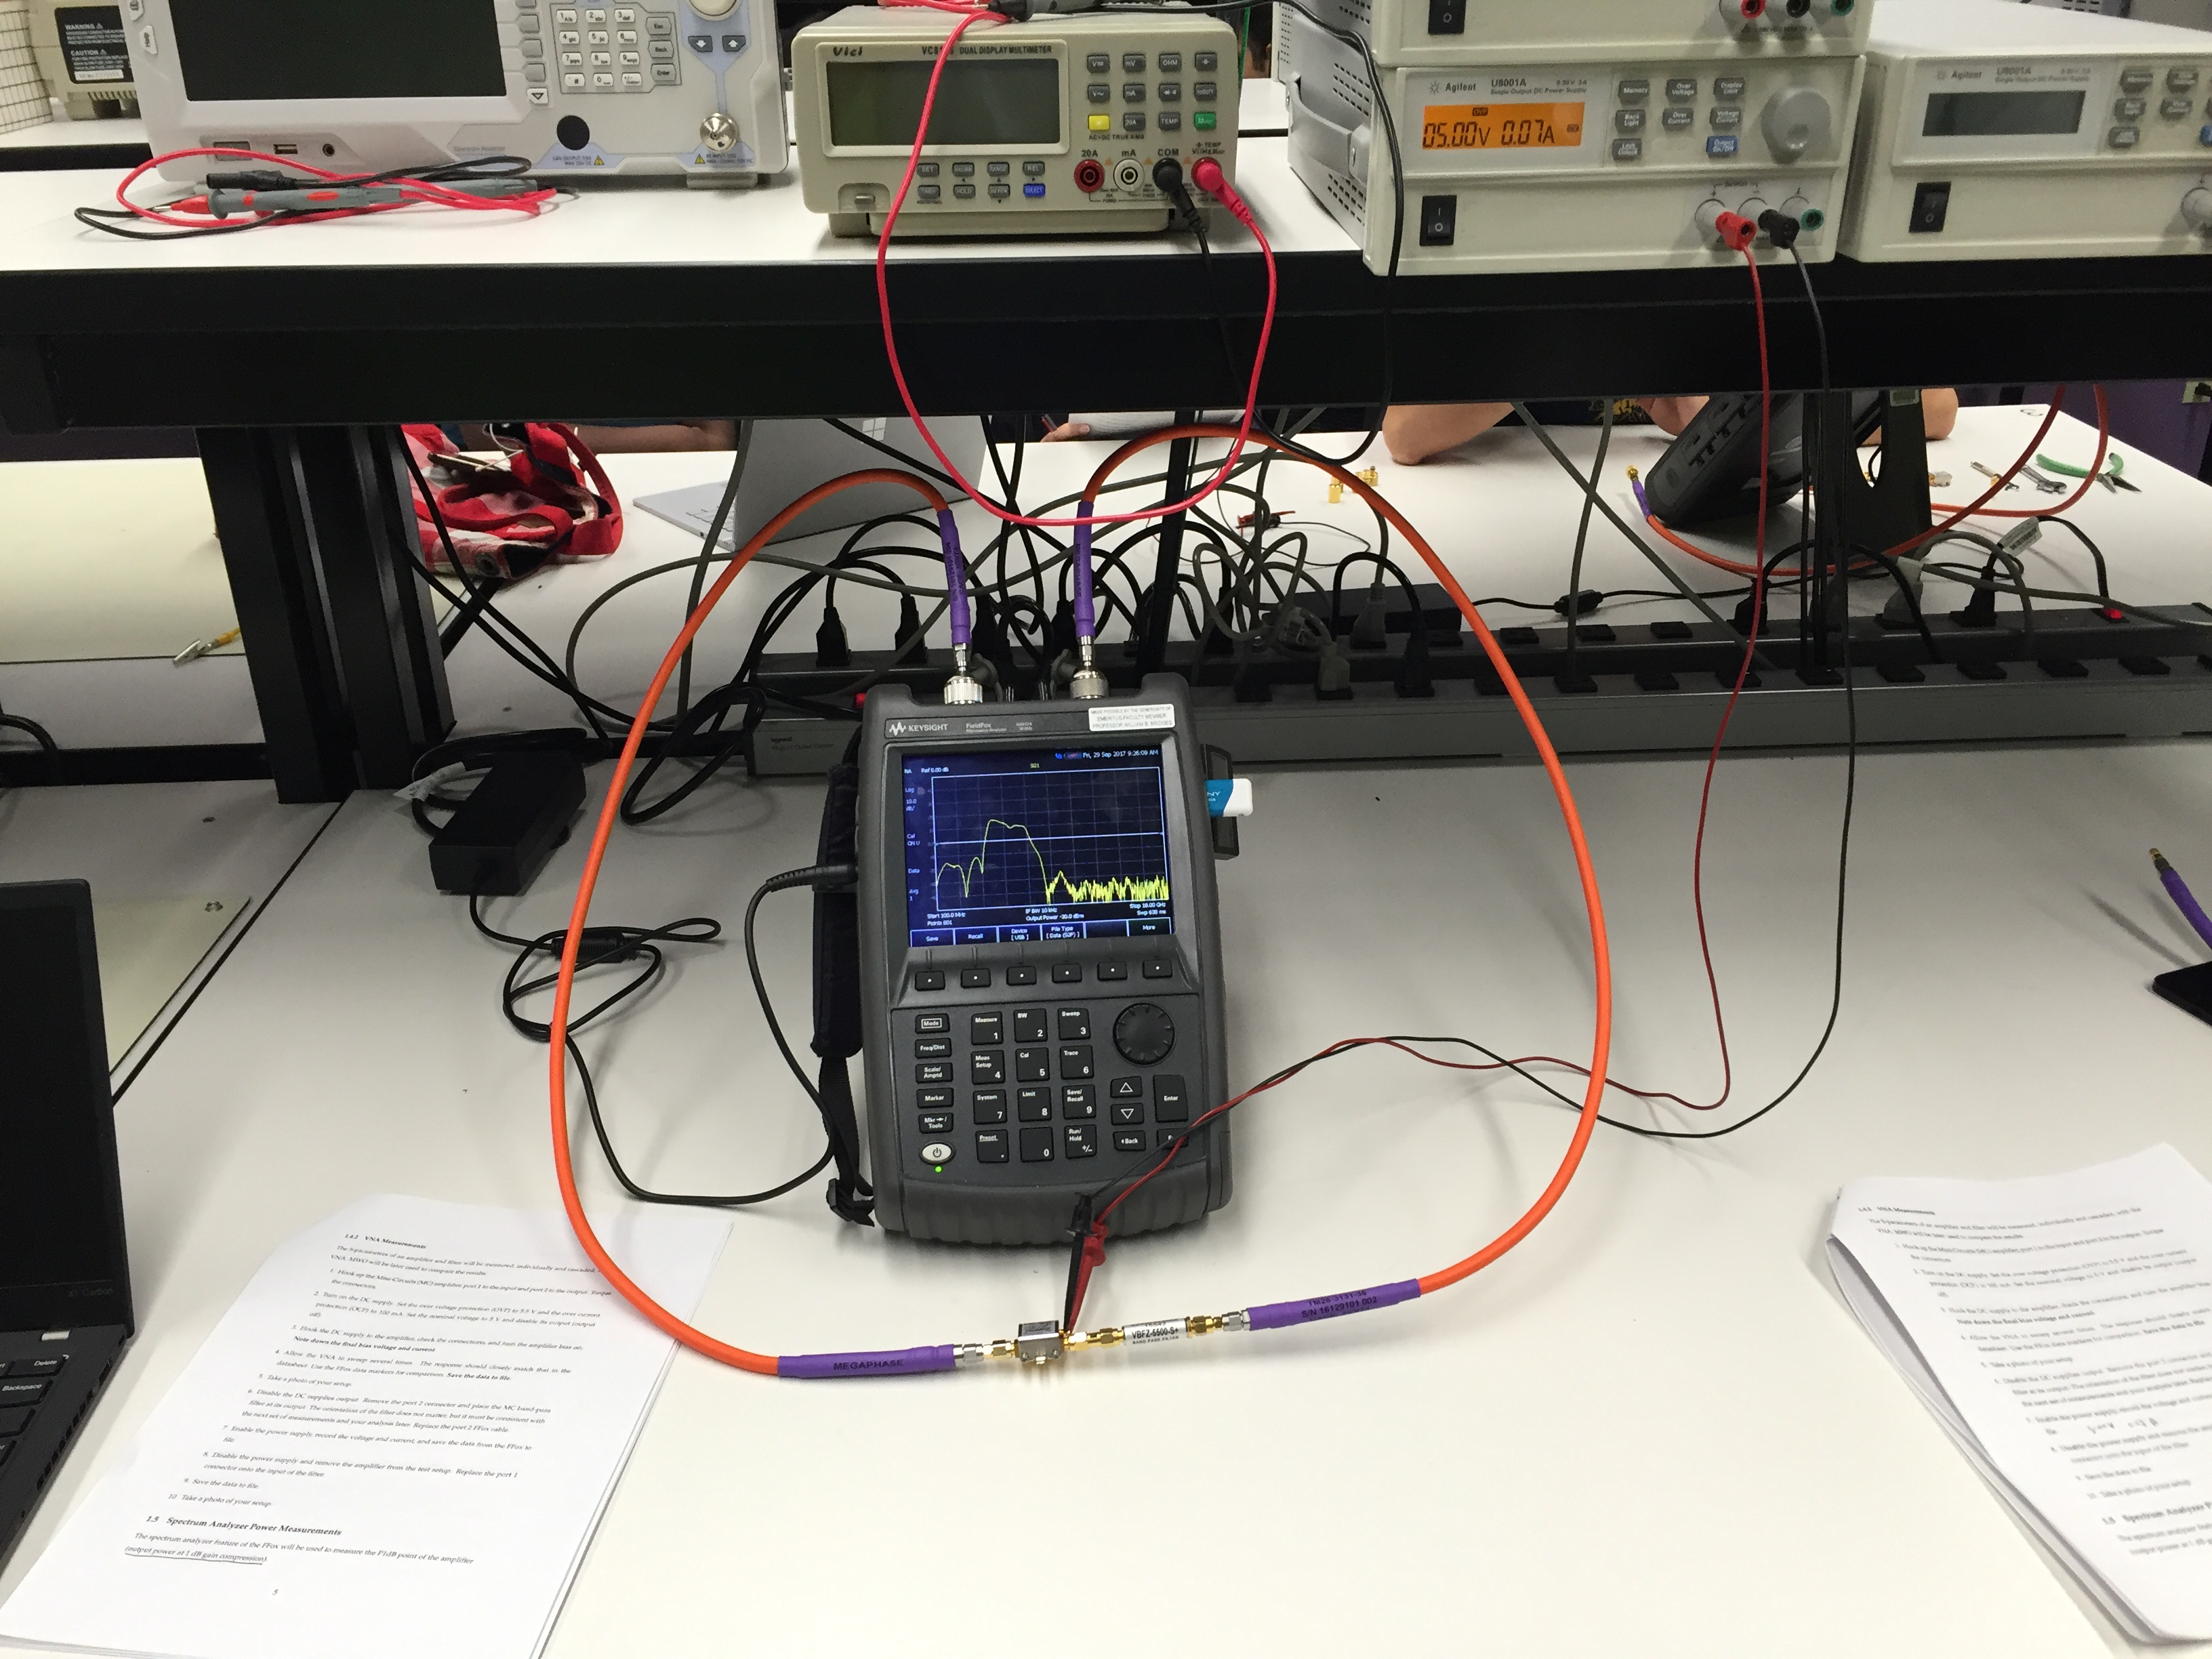
\includegraphics[width=0.35\textwidth]{amp_and_filter_measurement.jpeg}
    \caption{Measurement Setup for amplifier and filter circuit on the NA.}
    \label{fig:filtampimg}
\end{figure}

\begin{figure}[!htbp]
    \centering
    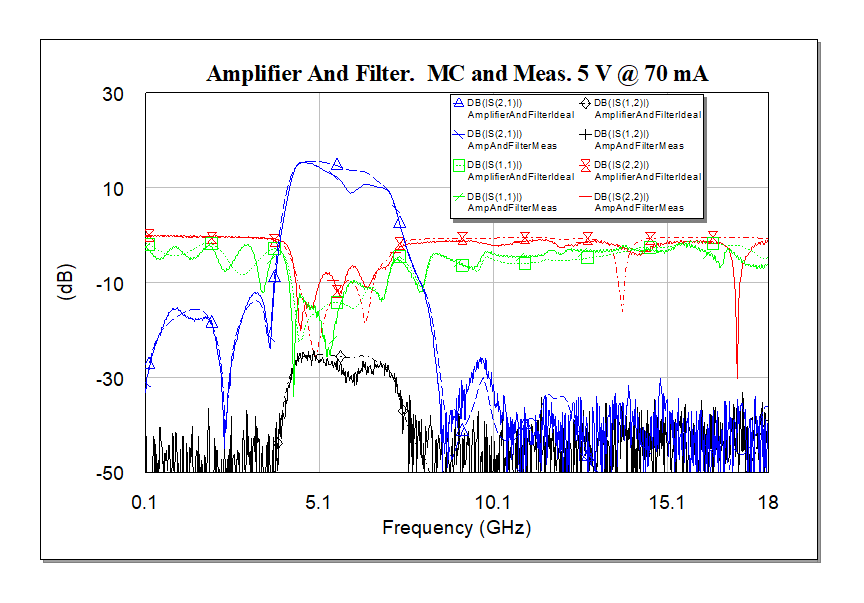
\includegraphics[scale=0.45]{AmpAndFilterMCandMeasured.png}
    \caption{Comparison of the Amplifier and Filter circuit S parameters from the NA measurements to the simulated parameters.}
    \label{fig:ampfilter}
\end{figure}

\FloatBarrier

\section*{Spectral Measurements}

In order to correctly measure the input power vs. output power response of the MC amplifier, we needed to first quantify the losses in the circuit due to the cabling and connectors. To do so, we connected a signal generator through the SMA cables to the SA and measured the power in the SA as a function of the power from the signal generator. We swept Pin from -20.0 dBm to 0.0 dBm in 1 dB steps. The results are shown in figure \ref{fig:cableloss}. This shows that we have about 2dB loss due to the cables.

\begin{figure}[!htbp]
    \centering
    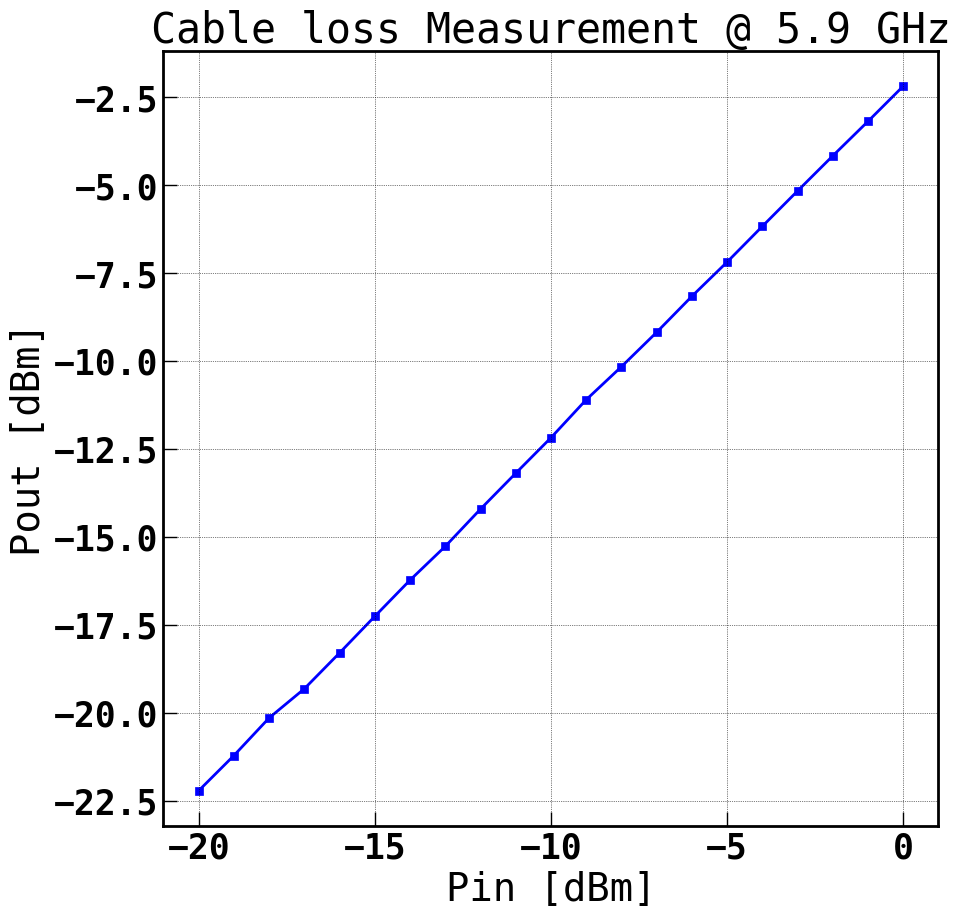
\includegraphics[scale=0.35]{cable_power_loss.png}
    \caption{Measurements of the Input Power from signal generator to the actual power measured. This shows the power loss in the cables and connectors.}
    \label{fig:cableloss}
\end{figure}

Once the amplifier is connected in the circuit as shown in figure \ref{fig:ampspectralimg}, we measured the output power of the amplifier as a function of the input power from the signal generator, adjusted for losses in the cables. In addition, a 10dB attenuator was added to the output of the amplifier to protect the SA from damage. This value was added back to the power measured by the SA. The signal generator provided a single tone at 5.9 GHz. At low input powers, the response of the amplifier is mostly linear as is shown in figure \ref{fig:ampcompress}. At higher input power, the amplifier saturates and delivers less power at 5.9 GHz than the expected linear response. This deviation is due to non-linearities becoming more and more important in the amplifier. From this, we measured the 1dB compression point of the amplifier as at an output power of 10.9 dBm at 5.9 GHz. The datasheet reports a 1dB compression point of 12.1 dBm at 6.00 GHz in contrast.

\begin{figure}[!htbp]
    \centering
    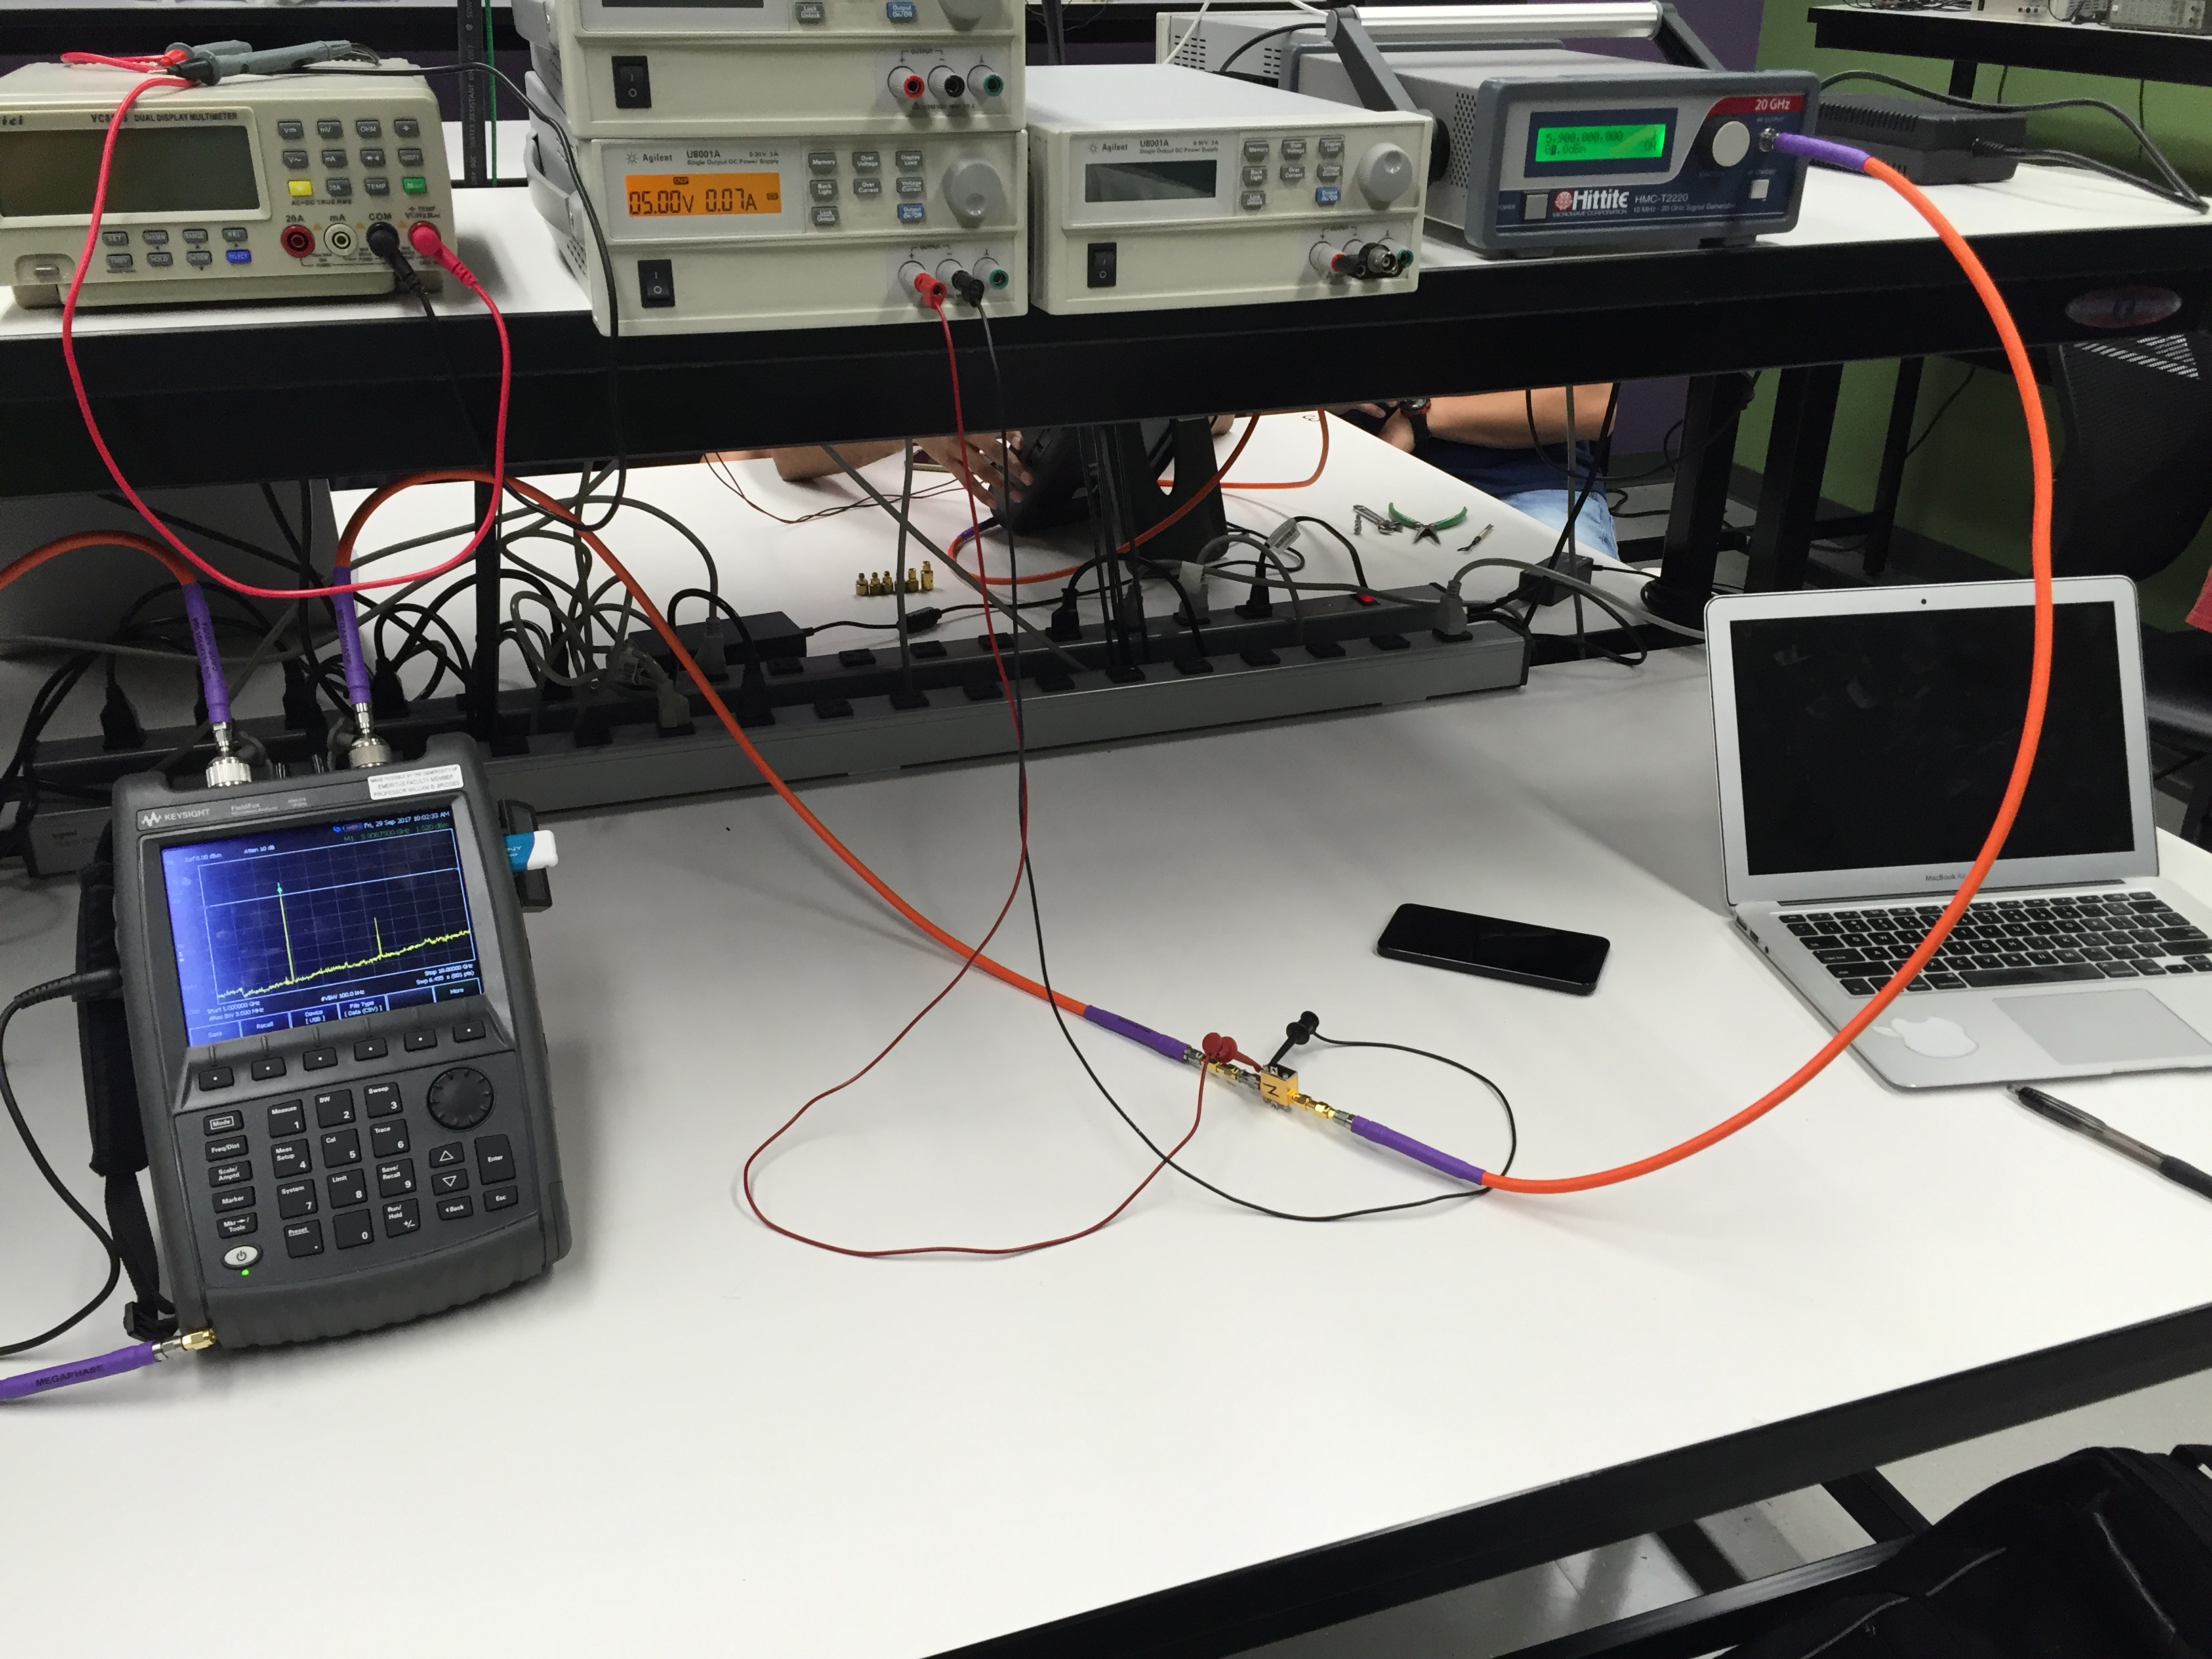
\includegraphics[width=0.35\textwidth]{amp_spectral_measurement.jpeg}
    \caption{Measurement Setup for amplifier on the SA. The fundamental and first harmonic are visible in the SA display.}
    \label{fig:ampspectralimg}
\end{figure}

\begin{figure}[!htbp]
    \centering
    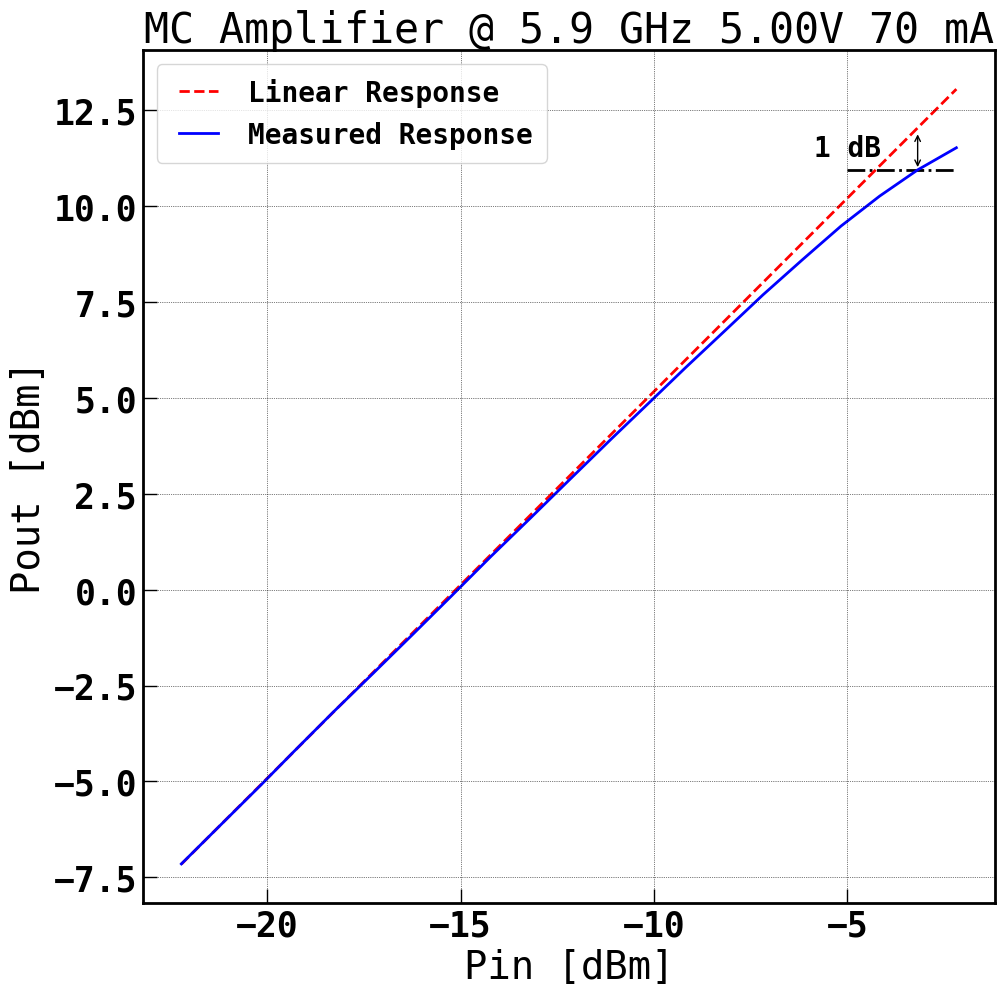
\includegraphics[scale=0.35]{amp_power_compression.png}
    \caption{Amplifier power response. The linear response over the entire input power range has also been plotted for comparison.}
    \label{fig:ampcompress}
\end{figure}

As described in the introduction section, the drop in response is due to the excitation of higher order harmonics that move power away from the fundamental. This can be clearly seen in the spectral traces of the amplifier at input power of -20.0 dBm vs. 0.0 dBm as shown in figure \ref{fig:spectra}. At low input power, only the fundamental tone is visible above the noise floor and at high SNR. At higher input power levels the second harmonic at 11.8 GHz is also clearly visible above the noise floor of the instrument.

\begin{figure}[!htbp]
    \centering
    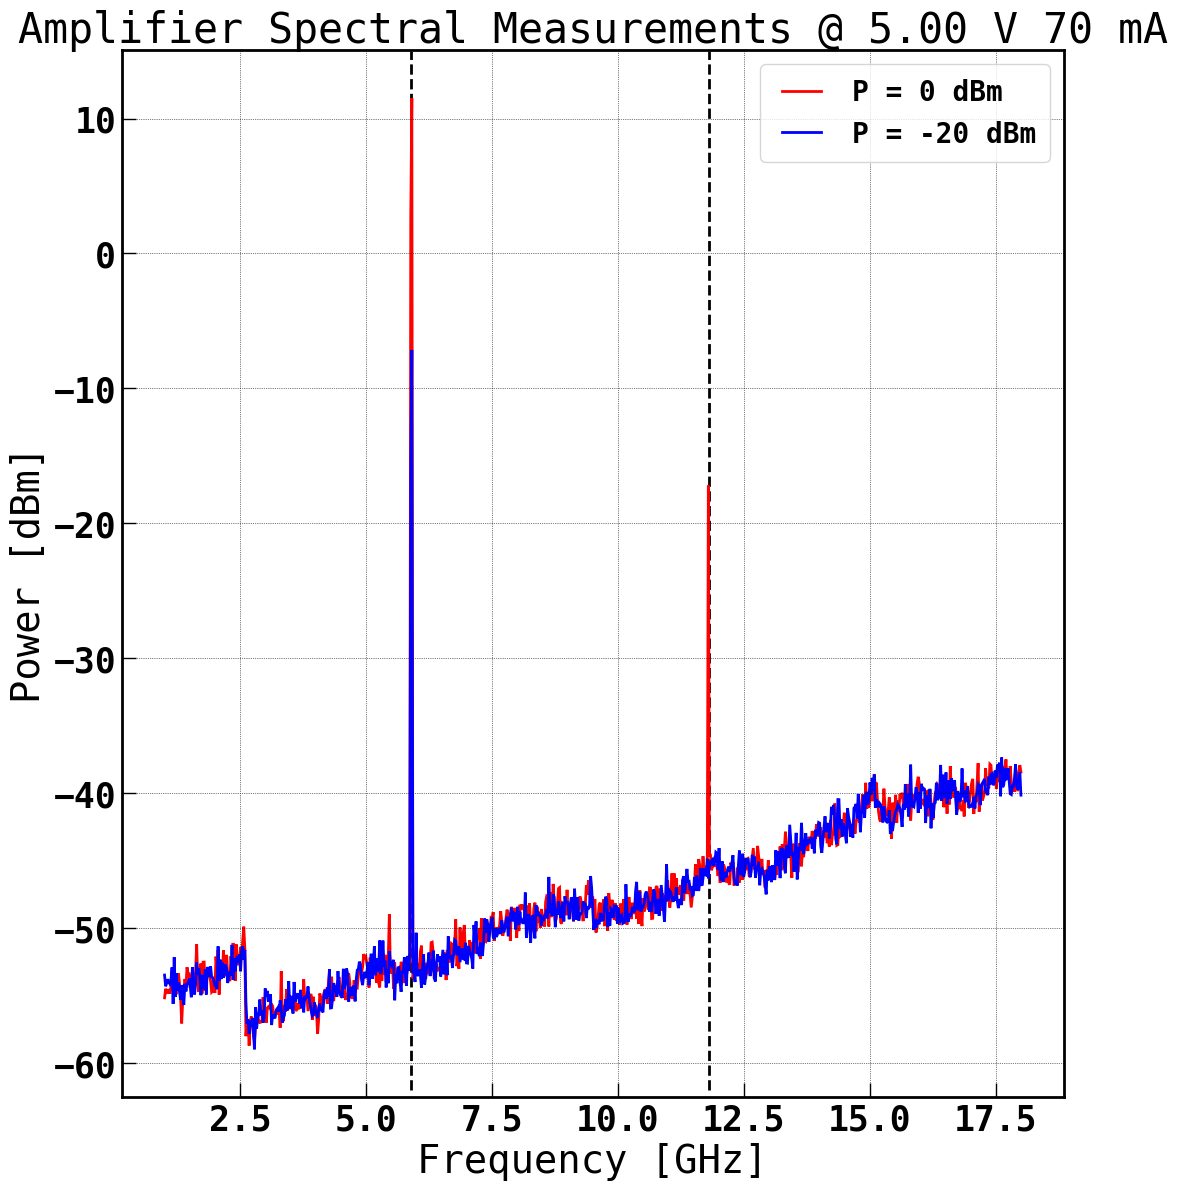
\includegraphics[scale=0.30]{spectra_20dB_vs_0dB.png}
    \caption{A plot of the amplifier spectrum with Pin = -20.0 dBm vs 0.0 dBm. The fundamental harmonic is at 5.9 GHz. At 0.0 dBm, the first harmonic at 11.8 GHz is visible.}
    \label{fig:spectra}
\end{figure}

\section*{Conclusions}
At the end of this document, I have also attached the code used to generate the plots for the SA measurements. The biggest takeaways from this lab were the fundamentals of using a Network Analyzer to perform measurements of the S parameters. I learned how to interpret the NA results and compare them with datasheet specifications using Microwave Office. I also learned how to chain different S parameter files to simulate the combined response of the total network. The use of Spectral Analyzers to investigate the non-linearities of amplifiers was also a key aspect of this lab. My suggestion for improvement would be better guidance on exactly what is expected in the lab reports. I spent a lot of time writing this one up.
\end{document}